	%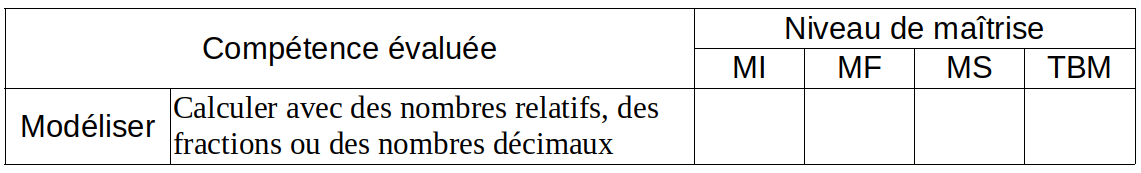
\includegraphics[scale=0.4]{competences}
	
	\section{Calculer}
	Calculer les expressions suivantes en détaillant tous les calculs:
	\begin{questions}
		
		\question[3]  $A =  44 + 37 - 15 + 28$
		
		\fillwithdottedlines{6cm}
		{\LARGE \begin{solution}
			\begin{eqnarray*}
				A &=& 44 + 37 - 15 + 28 \\
				A &=& 81 - 15 + 28 \\
				A &=& 66 + 28 \\
				A &=& 94
			\end{eqnarray*}
		\end{solution}}
		
		
		\question[3]  $B = (7 + 5) \times (8 - 2)$
		
		\fillwithdottedlines{6cm}
		{\LARGE \begin{solution}
			\begin{eqnarray*}
			B &=& (7 + 5) \times (8 - 2)\\
			B &=& 12 \times 6 \\			
			B &=& 72
			\end{eqnarray*}
		\end{solution}}
		
		\newpage
		\question[4]  $C =  44 + (37 - 15) + 28$
		
		\fillwithdottedlines{5cm}
		{\LARGE \begin{solution}
			\begin{eqnarray*}
			C &=&  44 + (37 - 15) + 28\\
			C &=&  44 + 22 + 28\\
			C &=& 66 + 28\\
			C &=& 94
			\end{eqnarray*}
		\end{solution}}
		
		 \question[4]  $D = (50 - (13 + 1) \times 2) - 6$
		
		\fillwithdottedlines{5cm}
		{\LARGE 
			\begin{solution}
			\begin{eqnarray*}
			D &=&  (50 - (13 + 1) \times 2) - 6\\
			D &=&  (50 - 14 \times 2) - 6\\
			D &=& (50 - 28) - 6\\
			D &=& 22 - 6 \\
			D &=& 16 
			\end{eqnarray*}
		\end{solution}}
		
%		{\LARGE \question[2]  $E = (19 - 7 \times 2) + 4$}
%		
%		%\fillwithdottedlines{6cm}
%		{\LARGE \begin{solution}
%			\begin{eqnarray*}
%			E &=&  (19 - 7 \times 2) + 4\\
%			E &=&  (19 - 14) + 4\\
%			E &=& 5 + 4 \\
%			E &=& 9 
%			\end{eqnarray*}
%		\end{solution}}
	\end{questions}


\section{Traduire}
Traduire les expressions suivantes par une phrase, sans faire les calculs.
\begin{questions}
	
	\question[3]  $E = 63 - 45 \div 7$
	\fillwithdottedlines{3cm}
	
	
	\question[3]  $F = (73 \div 5) \times (24 + 9)$
	\fillwithdottedlines{3cm}
\end{questions}
	
	
